\documentclass[12pt]{article}

\usepackage[utf8]{inputenc}
\usepackage[francais]{babel}
\usepackage{amsmath}
\usepackage{url}
\usepackage{float}
\usepackage{graphicx}
\usepackage{subfigure}

\title{Recherche de chemin par dépôt de phéromones}
\author{Merwan Achibet $\;$ \textendash $\;$ Université du Havre}
\date{}

\begin{document}

\maketitle

\section*{Introduction}

On se propose d'étudier l'implémentation NetLogo de José M. Vidal
inspirée de \textit{Synthetic Pheromone Mechanisms for Coordination of
  Unmanned Vehicles} de Parunak, Brueckner et Sauter. Dans un premier
temps, on étudie le modèle original puis on analyse l'implémentation
fournie.

\section{Le modèle}

\subsection{Analogie avec le vivant}

Les fourmis sont des insectes reconnus pour leur caractère
social. Seules, elles restent vulnérables à l'environnement immense
les entourant. Pourtant, la coopération entre individus de la même
colonie caractérisant cette espèce leur permet de compter parmi les
êtres vivants les plus présents sur le globe terrestre.

Les fourmis communiquent par le biais de signaux chimiques que l'on
peut assimiler à des odeurs, les phéromones \cite{insectes}. Elles
peuvent dialoguer d'individu à individu en utilisant leurs antennes
mais, dans le contexte de la croissance de la fourmilière, il est plus
efficace de déposer dans leur environnement des messages généraux
adressés à tous. C'est notamment le cas lorsqu'une nouvelle source de
nourriture est trouvée puisque la fourmi à l'origine de l'heureuse
découverte déposera derrière elle des phéromones de piste afin que ses
congénères puissent y être guidées. Plusieurs autres types de
phéromones existent : certaines préviennent d'un danger tandis que
d'autre délimitent un territoire ou bien, chez d'autres espèces,
attirent les individus de sexe opposé en période de reproduction.

Les phéromones étant des signaux chimiques éphémères, un phénomène
d'évaporation se produit naturellement et efface progressivement les
pistes.  Pour qu'une piste perdure, elle doit être entretenue par
accumulation des phéromones des autres fourmis l'arpentant. Ainsi
seules les meilleures pistes sont conservées tandis que les autres
(sources de nourriture épuisées ou moins importantes) disparaissent
par érosion.  Un aspect important des phéromones est qu'elles sont
soumises à une diffusion dans l'environnement et que les insectes
disposent d'un odorat assez fin pour en retrouver la source. Ainsi, un
individu peut détecter et être attiré par une odeur en passant à
proximité de la piste originelle mais sans nécessairement la croiser.

Ce type de comportement est une source d'inspiration pour la
conception de méthodes de résolution destinée à des systèmes
multi-agents puisqu'il rassemble des qualités notables \cite{dorigo}
:

\begin{description}
\item[Diversité]{Une phéromone peut aussi bien indiquer une piste à
  suivre qu'un danger. Le concepteur d'un modèle est libre d'associer
  tout type de sémantique à une phéromone.}
\item[Distribution]{Les signaux chimiques guidant les insectes sont
  répartis sur tout l'environnement.}
\item[Décentralisation]{Si une fourmi est mangée par un oiseau, cela
  n'impactera pas l'avenir de la fourmilière car l'individu manquant
  n'est qu'un rouage d'un mécanisme plus complexe et les signaux qu'il
  a déposés perdureront jusqu'à évaporation.}
\item[Dynamicité]{Les tracés se renforçant et s'évaporant
  continuellement, les insectes s'adaptent à tout changement impromptu
  de l'environnement.}
\end{description}

Parunak \textit{et al.} partent de ce constat, et s'inspirent des
modèles existants \cite{swarm}, pour proposer une méthode de guidage
destinée aux véhicules non habités dans le cadre d'opérations
militaires.

\subsection{Les agents et leur monde}

Ici, la fourmi est remplacée par un véhicule, un drone aérien dans
l'exemple. Sa mission est de partir d'une base et d'atteindre un
bâtiment ennemi cible tout en évitant certaines infrastructures
pouvant l'impacter négativement (radars, batteries anti-aérienne). La
figure \ref{real} montre un exemple de configuration réalisable.

\begin{figure}[H]
  \centering

  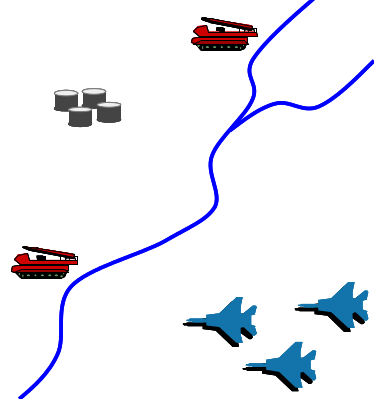
\includegraphics[width=6.5cm]{terrain_real.png}

  \caption{Exemple de configuration modélisable. En bleu, les drones;
    en gris, la cible; en rouge les menaces \cite{parunak}.}
  \label{real}
\end{figure}

Tout d'abord, l'environnement est divisé en zones (\textit{places})
dont les dimensions dépendent de la simulation envisagée.  Dans
l'exemple \textit{SEADy Storm} proposé dans le papier étudié, une zone
correspond à un hexagone de 50 kilomètres de diamètre. C'est sur ces
zones que les quantités des différentes phéromones déposées par les
acteurs de la simulation sont stockées et que le phénomène de
diffusion se produit entre zones voisines.

L'acteur principal, le véhicule, peut déposer deux types de phéromones
:

\begin{description}
\item[GNest]{Libérée par un agent venant de quitter la base. Elle
  guide les autres agents vers la base.}
\item[GTarget]{Libérée par un agent venant de rencontrer une cible
  ennemi et rentrant à sa base. Elle guide les autres agents vers la
  cible.}
\end{description}

Dans ce modèle, les bâtiments ennemis sont eux aussi agents et
émetteurs des phéromones :

\begin{description}
\item[RTarget]{Libérée par les bâtiments cibles. Elle attire les
  drones.}
\item[RThreat]{Libérée par les bâtiments de contre-mesure. Elle
  repousse les drones.}
\end{description}

Chacune de ces phéromones véhicule une information différente, mais au
delà de leur sens, elles différent aussi de par leur taux de diffusion
dans l'environnement.  Pour les bâtiments ennemis, ce taux de
diffusion dépend de l'aire d'effet du bâtiment associé, et correspond
concrètement à son rayon d'action : le rayon de détection pour un
radar, la portée pour une batterie anti-aérienne.  Le taux de
diffusion des phéromones libérées par les drones doit quant à lui être
finement mesuré pour que les pistes soient remarquées par les
véhicules passant à proximité sans pour autant définir une route trop
large et donc plus encline à empiéter sur les aires d'effet des
bâtiments ennemis.

Le fonctionnement intrinsèque de ce modèle commence à s'esquisser. Les
phéromones émisent par les différents acteurs de la simulation vont
tisser un canevas de signaux chimiques marquant l'environnement.
Typiquement, les drones auront pour but de suivre une piste menant à
un bâtiment cible tout en évitant les aires d'effet des bâtiments
menaçants, puis à revenir jusqu'à une base. La figure \ref{field}
illustre la configuration de la figure \ref{real} de ce point de vue.

\begin{figure}[H]
  \centering

  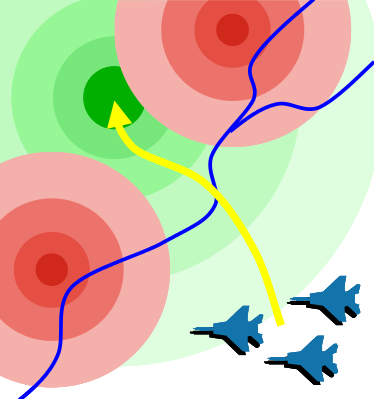
\includegraphics[width=6.5cm]{terrain_field.png}

  \caption{Le même environnement marqué par les phéromones des
    bâtiments ennemis \cite{parunak}.}
  \label{field}
\end{figure}

\subsection{Guidage}

Les phéromones décrites sont bien sûr spécifiques au modèle présenté
et on peut aisément imaginer, selon la simulation, que l'on en
introduise de nouveaux types. Dans un soucis de généralisme et de
simplicité, on ne souhaite pas qu'un agent ait à envisager des
considérations complexes prenant en compte chaque phéromones
séparement et on préfère associer aux zones une fonction $g$ calculant
une valeur d'attractivité nette afin de guider le déplacement des
drones. Dans l'exemple proposé, cette fonction est la suivante, avec
$\alpha$, $\beta$, $\gamma$, $\delta$ et $\theta$ des facteurs de
réglage et $\operatorname{Dist}$ une approximation de la distance
séparant le drone de sa cible :

\begin{equation}
  g = \frac{ \theta \operatorname{RTarget} + \gamma
  \operatorname{GTarget} + \beta}{\alpha \operatorname{RThreat} + \delta
  \operatorname{Dist} + \beta}
  \label{g}
\end{equation}

Lorsqu'un véhicule se trouve dans une zone, il a accès aux quantités
de phéromones présentes dans les zones voisines et un tirage aléatoire
de type roue de la fortune biaisée permet de simuler un choix quant à
la route à emprunter. Plus une zone est attractive (beaucoup de
phéromones menant à la cible, peu de phéromones menant à une menace)
et plus la probabilité de l'emprunter est elevée.

Généralement, et si le drone suit déjà une piste et qu'il est aligné
sur sa direction, les zones les plus attrayantes se trouvent devant et
derrière lui. Afin d'éviter qu'il ne change intempestivement de
direction et prenne la piste à l'envers, son élan est pris en compte
et la zone directement dans le sens de son déplacement bénéficie d'un
bonus lors du tirage aléatoire.

Pour l'instant, seuls les agents mobiles de type drone ont été
présentés. Il en existe pourtant une seconde catégorie, qui peuple en
majorité l'espace de la simulation et que nous appellons les
fantômes. Un fantôme est un drone virtuel à courte durée de vie et à
courte portée, lâché par le véritable drone, et donc la principale
caractéristique est de disposer d'une vitesse d'exploration plus
importante.  Les fantômes se comportent de la même façon que leur
drone parent vis à vis des phéromones; elles servent à leur guidage et
ils les déposent sur leur chemin. Ils font ainsi office d'éclaireurs
et améliorent les choix de déplacement du véritable drone en évaluant
par avance les choix qui s'offriront à lui (voir figure \ref{ghosts}).

\begin{figure}[H]
  \centering

  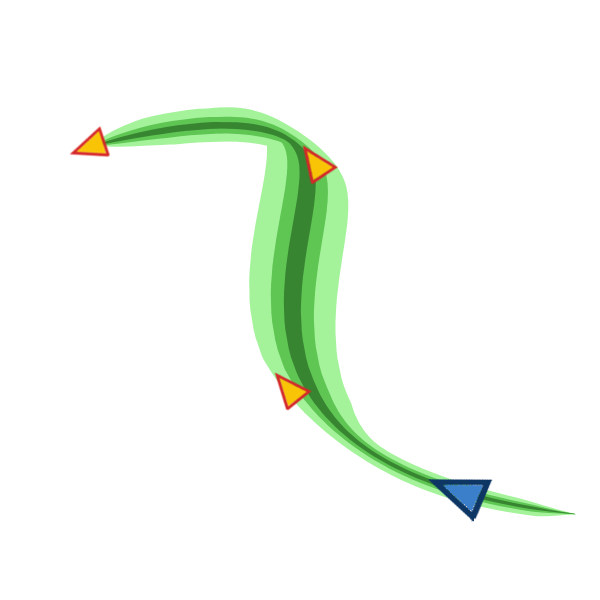
\includegraphics[width=8cm]{ghosts.png}

  \caption{Un drone (en bleu) suit la piste de phéromones (en vert)
    déposée et renforcée par ses fantômes (en orange).}
  \label{ghosts}
\end{figure}

Le concept des fantômes est une différence majeure entre la méthode
proposée et un algorithme de colonies de fourmis classique. Il est
bien sûr plus adapté au cadre opérationnel décrit, car l'action d'un
drone doit être rapide et efficace. On imagine mal que le travail
d'exploration de tout l'espace aérien revienne au drone. L'utilisation
d'éclaireurs, plus rapides et de plus petite taille, est donc
justifiée.

\section{L'implémentation}

\subsection{\'Etude}

L'implémentation de Vidal est basée sur une grille torique de
\textit{patches} carrés alors que l'implémentation originale utilisait
des hexagones. Cette différence est négligeable au niveau des
résultats que fournit cette simulation car Parunak \textit{et al.}
précisent que la configuration du terrain et des blocs le formant,
ainsi que leurs dimensions, peuvent varier librement.

Chaque \textit{patch} contient une valeur réelle représentant le
volume de chacune des phéromones qu'il contient. La diffusion de ces
signaux chimiques se fait par la fonction NetLogo \texttt{diffuse} qui
partage une fraction de la phéromone entre les huit zones
adjacentes. L'évaporation est réalisée manuellement et la valeur de
chaque phéromone est réduite à chaque itération d'un pourcentage
réglable. Un exemple de configuration est visible sur la figure
\ref{pheromones}.

\begin{figure}[p]
  \centering

  \mbox{
    \subfigure{
      \subfigure[RTarget]{
        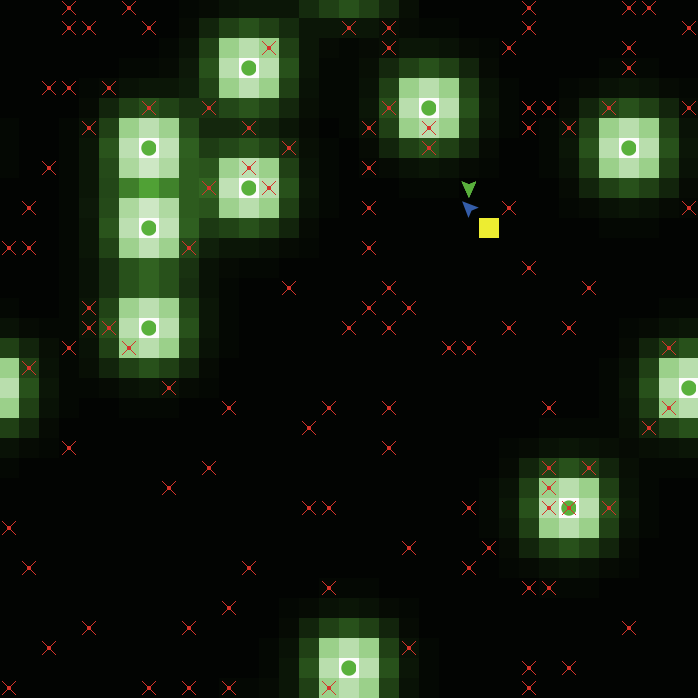
\includegraphics[width=6.5cm]{pheromones_target.png}
      }
      \quad
      \subfigure[RThreat]{
        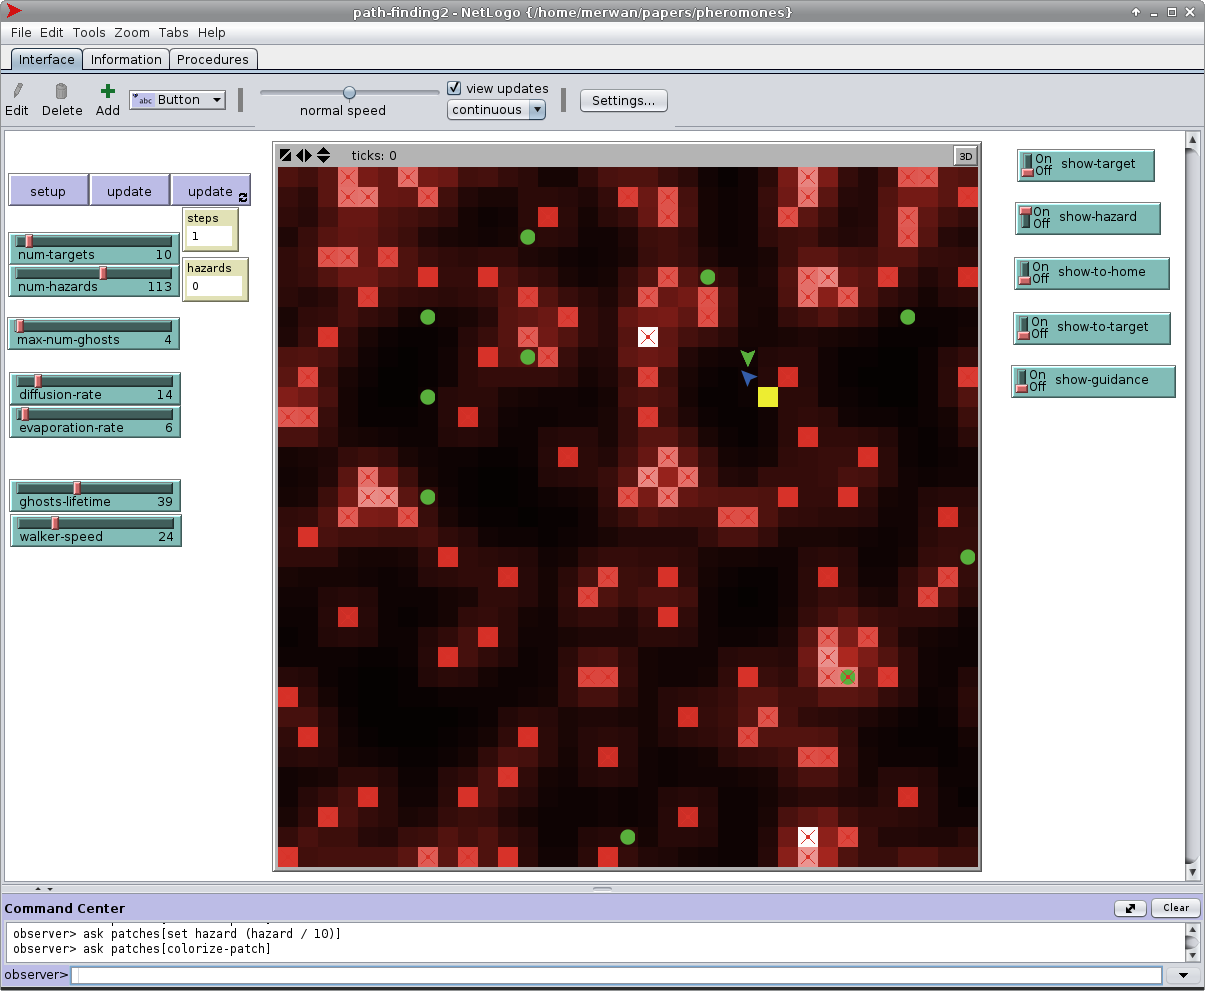
\includegraphics[width=6.5cm]{pheromones_hazard.png}
      }
    }
  }
  \mbox{
    \subfigure{
      \subfigure[GTarget]{
        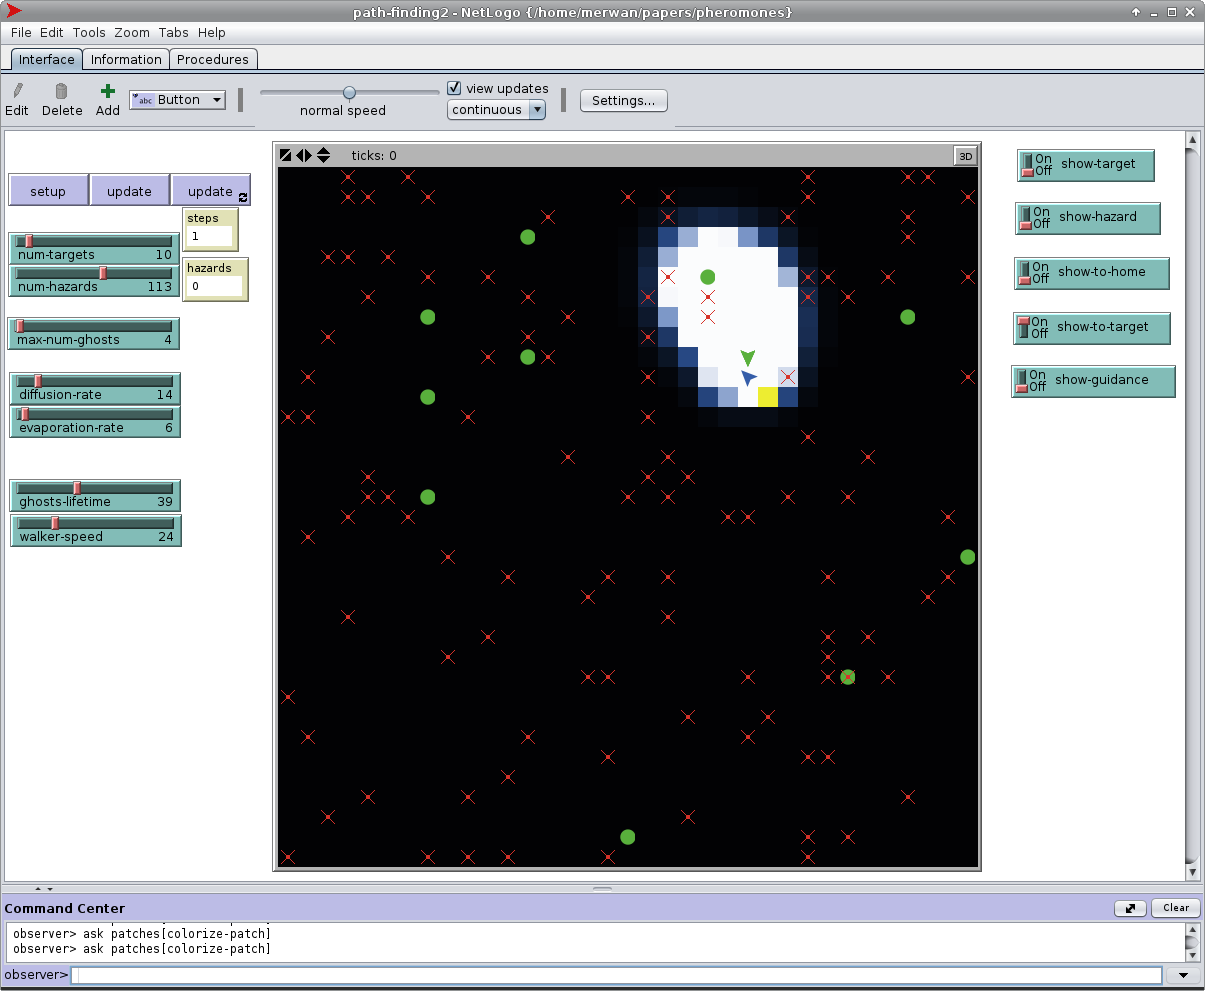
\includegraphics[width=6.5cm]{pheromones_totarget.png}
      }
      \quad
      \subfigure[GNest]{
        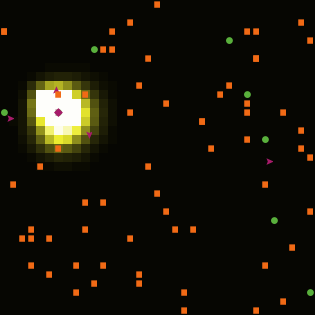
\includegraphics[width=6.5cm]{pheromones_tohome.png}
      }
    }
  }

  \caption{Les quatre types de phéromone pour une configuration
    donnée. En violet, les drones; en vert les cibles; en orange, les
    menaces; en jaune, la phéromone.}
  \label{pheromones}
\end{figure}

La simulation comprend un unique drone physique et se termine lorsque
ce dernier atteint une des cibles. Ce véhicule ayant ici pour unique
but de toucher l'objectif, il ne fait que se déplacer de
\textit{patch} en \textit{patch} en utilisant comme heuristique la
quantité de phéromone GTarget (menant à une cible) des cases voisines,
via la fonction NetLogo \texttt{uphill}. L'équation \ref{g} n'est donc
pas utilisée. En conséquence, le drone se dirige vers les cibles sans
prêter attention aux menaces ennemies, l'interêt de la simulation en
est donc fortement réduit puisque l'évitement des menaces est un des
principaux intérêts du modèle.

On retrouve dans cette implémentation le fait que les fantômes
disposent d'une vitesse plus elevée que leur drone parent afin
d'explorer en avance l'espace de la simulation. Ici, une itération de
la simulation correspond à un déplacement de fantôme. Le véritable
drone se déplace tous les $n$ pas de fantômes ($n$ est réglable par
l'utilisateur).

Les fantômes sont instanciés par le drone principal dés le début de la
simulation. \`A chaque fois qu'un drone est arrivé à la fin de sa
durée de vie, un nouveau est ajouté à la position du drone. Ils
oscillent entre deux modes :

\begin{description}

  \item[to-target]{Dans ce mode, ils se dirigent vers une cible en
    suivant les phéromones de type RTarget (libérées par les cibles)
    et lâchent des phéromones de type GNest (menant à la base). Les
    déplacements se font de la même façon que pour les drones
    physiques, via \texttt{uphill}. La formule \ref{g} n'est pas non
    plus utilisée ici. On passe au second état quand une cible est
    atteinte.}

  \item[to-home]{Dans ce mode, ils reviennent à la base en suivant les
    phéromones de type GNest et libèrent des phéromones de type
    GTarget menant à la dernière cible visitée.}

\end{description}

On remarque que \textbf{to-target} est le mode initial d'un
fantôme. La phéromone déposée pendant cet état guide donc en fait vers
leur position de naissance et non vers une véritable base physique
(zone d'atterissage par exemple). Position de naissance correspondant
en fait à la position de leur drone parent puisque les fantômes sont
plus rapides et il est donc possible qu'ils atteignent une cible puis
repassent par la position du drone parent avant même que ce dernier ne
se soit déplacé. Ce choix peut être justifié par le fait que dans une
situation réelle, les fantômes pourraient correspondre à de minuscules
appareils utilisant leur drone parent, un véhicule plus imposant,
comme base mobile.

\subsection{Analyse}

Les facteurs que l'utilisateur peut contrôler sont :

\begin{itemize}
\item{Le nombre de cibles}
\item{Le nombre de menaces}
\item{Le taux de diffusion des phéromones}
\item{Le taux d'évaporation des phéromones}
\item{Le nombre de fantômes}
\item{La durée de vie d'un fantôme}
\item{La vitesse du drone}
\end{itemize}

On remarque que le taux de diffusion ainsi que le taux d'évaporation
est commun à toutes les phéromones, contrairement au modèle original
qui supporte les phéromones disposant de dynamiques différentes.

Comme suggéré précédemment, cette implémentation n'est pas assez
fidèle au modèle original pour que les résultats soient
significatifs. Le principaux défaut étant un guidage simplifié ne
prenant pas en compte les obstacles à éviter.

On peut néanmoins faire varier quelques paramètres et remarquer
plusieurs résultats. Premièrement, on note qu'un grand nombre de
fantômes diminue la durée de la recherche car plus de chemins sont
explorés et les pistes prometteuses sont plus rapidement renforcées.

On observe aussi qu'un taux de diffusion mal adapté peut grandement
perturber la simulation. S'il est trop faible, les pistes restent
linéaires et une fois qu'un fantôme en croise une, il la suit sans en
ressortir (notamment à cause de l'utilisation stricte de
\texttt{uphill} à la place de la formule \ref{g}). \`A l'inverse, un
taux de diffusion trop elevé inonde l'environnement de phéromones et
les drones errent sans qu'aucun chemin n'émerge.

De la même façon, le taux d'évaporation est à contrôler. S'il est trop
faible, les pistes ne persistent pas et le drone et les fantômes n'ont
pas le temps de les suivre. S'il est trop élevé, les pistes perdurent
trop longtemps, même si elles sont de mauvaise qualité, et induisent
les drones en erreur.

\subsection{Nouvelle version}

Comme montré précédemment, le défaut principal de cette implémentation
est dû au fait que \texttt{uphill GTarget} est utilisé pour suivre les
dépots de phéromone et s'approcher d'une cible. En conséquence, le
chemin est forcément le plus court (une ligne droite) mais il passe
indifférement sur des zones gardées ou non. On choisit de modifier le
programme NetLogo afin d'obtenir des résultats plus fidèles à ceux du
papier original.

Le c\oe ur du script est conservé. On ajoute uniquement à chaque
\textit{patch} un nouveau type de phéromone : la phéromone nette
calculée à l'aide de la formule \ref{g}. Elle est mise à jour pour
toutes les zones entre chaque itération de la simulation.

pour le guidage de chaque agent mobile, on procède comme suit :

\begin{enumerate}
  \item{On obtient la valeur de la phéromone nette de chacune des huit
  cases voisines à celle de l'agent}
  \item{On effectue un tirage aléatoire sur une roue dont les huit tranches
  sont biaisée en fonction de la valeur d'attractivité de la case
  associée}
  \item{On déplace l'agent sur la zone choisie}
\end{enumerate}

Drones et fantômes atteignent désormais leur but tout en évitant les
menaces ennemies.

\bibliographystyle{alpha}
\bibliography{sources}

\end{document}
